\documentclass[11pt]{scrartcl}
\usepackage[sexy]{evan}
\usepackage{float}

% %%%%%%%%%%%%%%%%%%%%%%
% %%     evan.sty     %%
% %%%%%%%%%%%%%%%%%%%%%%
%
% This file is licensed under the BOOST software license 1.0.
% This basically means you can do whatever you want with it,
% as long as any TeX source versions published
% include my name and this copyright notice.
% The compiled PDF itself is NOT required to have an attribution,
% although of course such attributions are greatly appreciated :D
% Here is the text of the license:
%
% Boost Software License - Version 1.0 - August 17th, 2003
%
% Copyright (c) 2020 Evan Chen [evan at evanchen.cc]
% https://web.evanchen.cc/ || github.com/vEnhance
%
% Permission is hereby granted, free of charge, to any person or organization
% obtaining a copy of the software and accompanying documentation covered by
% this license (the "Software") to use, reproduce, display, distribute,
% execute, and transmit the Software, and to prepare derivative works of the
% Software, and to permit third-parties to whom the Software is furnished to
% do so, all subject to the following:
%
% The copyright notices in the Software and this entire statement, including
% the above license grant, this restriction and the following disclaimer,
% must be included in all copies of the Software, in whole or in part, and
% all derivative works of the Software, unless such copies or derivative
% works are solely in the form of machine-executable object code generated by
% a source language processor.
%
% THE SOFTWARE IS PROVIDED "AS IS", WITHOUT WARRANTY OF ANY KIND, EXPRESS OR
% IMPLIED, INCLUDING BUT NOT LIMITED TO THE WARRANTIES OF MERCHANTABILITY,
% FITNESS FOR A PARTICULAR PURPOSE, TITLE AND NON-INFRINGEMENT. IN NO EVENT
% SHALL THE COPYRIGHT HOLDERS OR ANYONE DISTRIBUTING THE SOFTWARE BE LIABLE
% FOR ANY DAMAGES OR OTHER LIABILITY, WHETHER IN CONTRACT, TORT OR OTHERWISE,
% ARISING FROM, OUT OF OR IN CONNECTION WITH THE SOFTWARE OR THE USE OR OTHER
% DEALINGS IN THE SOFTWARE.
%%%%%%%%%%%%%%%%%%%%%%%%%%%%%%%%%%%%%%%%%%%%%%%%%%%%%%%%%%%%%%%%%%%%%%%%%%%%%
\usetikzlibrary{arrows}
\usetikzlibrary{calc}
\theoremstyle{plain}



\begin{document}
\title{Basic Triangle Centers}
\author{Jonathan Pei}
\subtitle{}
\maketitle

\begin{abstract}
    Triangle centers are an important facet of euclidean geometry.
    Often problems require an intricate understanding of the relationships between them.
\end{abstract}
\newpage
\tableofcontents
\newpage
\section{Concurrency}
    The fact that many of the following triangle centers exist can be surprising. We will establish a condition which will help us prove that these centers do in fact exist.
    %
        \begin{theorem}[Ceva's] 
            In $\triangle ABC$, points D, E, and F are on sides BC, AC, and AB respectively. $\frac{BD}{DC}\cdot \frac{CE}{EA}\cdot\frac{AF}{FB} = 1$, if and only if the segments AD, BE, and CF are concurrent.
            
        \end{theorem}
        
    % 
    \begin{proof}
        We will first show that the direct implication holds. Let the point of concurrency be X. We have the following area ratio 
        $$\frac{[ABD]}{[ADC]} = \frac{[XBD]}{[XDC]}=\frac{BD}{DC}.$$
        As you may know, this implies $$\frac{[ABD-XBD]}{[ADC-XDC]}=\frac{[ABX]}{[AXC]}=\frac{BD}{DC}.$$
        Similarly, for the other sides we have 
        $$\frac{[BCE-XCE]}{[BEA-XEA]}=\frac{[BCX]}{[BXA]}=\frac{CE}{EA}$$
        $$\frac{[CAF-XAF]}{[CFB-XFB]}=\frac{[CAX]}{[CXB]}=\frac{AF}{FB}.$$
        Multiplying these 3 equalities gives us 
        $$\frac{BD}{DC}\cdot \frac{CE}{EA}\cdot\frac{AF}{FB} = 1.$$
        We now prove the converse. For the sake of contradiction, assume that the three segments are not concurrent.
        Name the intersection of segments BE and CF X. Now intersect AX with BC at D'. From the given we have $\frac{BD}{DC}\cdot \frac{CE}{EA}\cdot\frac{AF}{FB} = 1.$
        And since AD', BE and CF are concurrent we also have $\frac{BD'}{D'C}\cdot \frac{CE}{EA}\cdot\frac{AF}{FB} = 1.$
        This implies $\frac{BD'}{DC}=\frac{BD}{DC}$. Since D' and D are both on segment BC, they must be the same point which is a contradiction. Thus, our original assumption 
        that the three segments were not concurrent was wrong.
    \end{proof} 
 
    \begin{exercise}
        Find a trigonometric form of Ceva's Theorem.
    \end{exercise}

\section{Circumcenter}
\begin{definition}
    The circumcenter is the center of the circle that passes through the vertices of a triangle. 
\end{definition}
\begin{remark}
    We don't need to verify that this exists because any three non-collinear points describe a circle, which by definition has a center.
\end{remark}

The circumcenter comes up a lot in problems, mainly because circles are very popular in geometry!
\begin{example}
    In $\triangle ABC$, the circumcircle $\omega$ is drawn and the tangent $\ell$ at $B$ is drawn. If $O$ is the center of $\omega$,
    show that the angle formed by $\ell$ and $\seg{BC}$ is half of $\angle BOC$.
\end{example}
\begin{soln}
    Let $\angle BOC = x$. Since $\triangle BOC$ is isosceles, $\angle OBC = 90-\frac{x}{2}$. $\ell$ is perpendicular to $\seg{OB}$ because it is tangent so 
    the angle formed by $\seg{BC}$ and $\ell$ is $90-(90-\frac{x}{2})=\frac{x}{2}$.
\end{soln}
\section{Centroid}
    
        \begin{definition}
            The centroid is the intersection of the medians of a \\triangle.
       \end{definition} 
    
       
    \begin{exercise}
        Verify that the centroid always exists.
    \end{exercise}
    Often the most important fact about the centroid used in computational
    contests is that the medians divide each other into a 2:1 ratio at the centroid.
    
        \begin{theorem}
            If AD,BE, and CF are medians in $\triangle ABC$ and G is the centroid then $$\frac{AG}{GD}=\frac{BG}{GE}=\frac{CG}{GF}=2$$
        \end{theorem}
    
    \begin{proof}
        Begin by drawing segment EF. We notice that $\triangle EFG \sim \triangle BGC$.
        So $\frac{BG}{GE} =2$. Likewise for the other medians finishes the proof.
    \end{proof}
    
        \begin{corollary}
        \label{median ratios}
            The 6 triangles formed by the medians and the sides of the triangle have equal area.
        \end{corollary}
    
    \subsection{Exercises}
    \begin{exercise}
        Prove corollary \ref{median ratios}.
    \end{exercise}
    \begin{exercise}[2018 AMC]
        Square $ABCD$ has side length $30$. Point $P$ lies inside the square so that $AP = 12$ and $BP = 26$. The centroids of $\triangle{ABP}$, $\triangle{BCP}$, $\triangle{CDP}$, and $\triangle{DAP}$ are the vertices of a convex quadrilateral. What is the area of that quadrilateral?
    \end{exercise}
    \begin{exercise} If D,E, and F are the midpoints of $\triangle ABC$ and G is the centroid, show that G is the centroid of $\triangle DEF$
    \end{exercise}
    \begin{exercise} AB is the diameter of a circle and C is a point on the circle. What shape does the centroid of $\triangle ABC$ trace as C moves around the circle.
    \end{exercise}

\section{Incenter}
\begin{definition}
    The incenter is the center of the circle which is tangent to all three sides of the triangle.
\end{definition}
If we show that the internal angle bisectors of a triangle always coincide, we prove that the incenter always exists along with the incircle.

\begin{exercise}
    Verify using Ceva's theorem that the incenter always exists.
\end{exercise}


\section{Orthocenter}

    \begin{definition}
        The orthocenter is the intersection of the altitudes of a triangle.
   \end{definition} 

\begin{exercise}
    Show that the orthocenter exists in all triangles. This is a simple application of trig Ceva.
\end{exercise}


\begin{figure}[H]
    \centering
    \scalebox{.75}{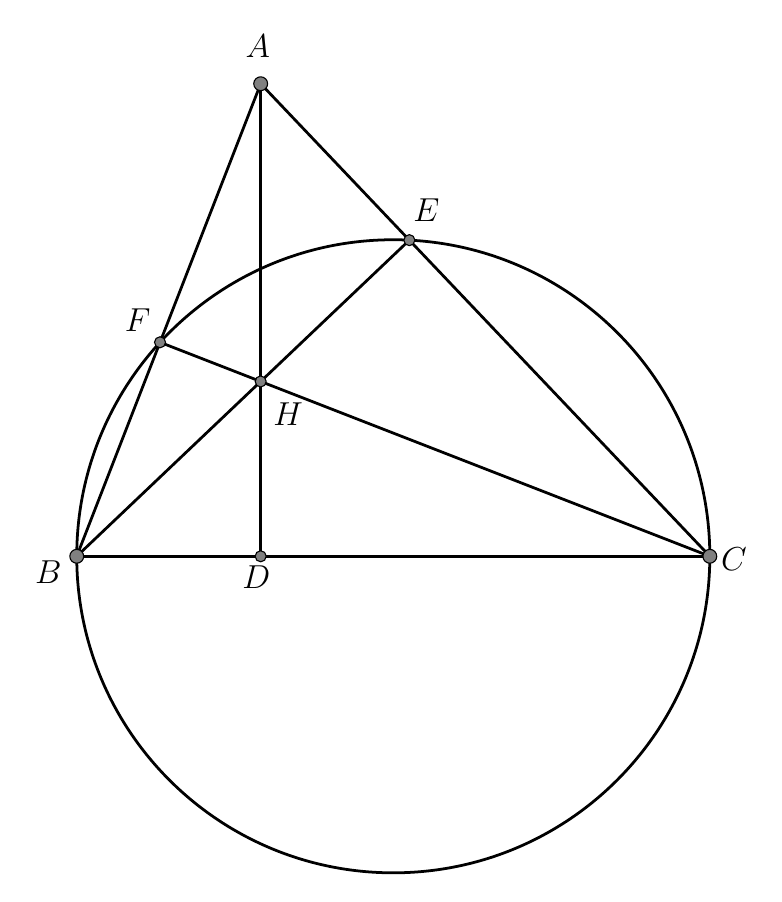
\begin{tikzpicture}[line cap=round,line join=round,>=triangle 45,x=1cm,y=1cm]
        \draw [line width=1pt,color=black] (-6.704024039828016,6.001415467595274)-- (-9.04,0);
        \draw [line width=1pt,color=black] (-9.04,0)-- (-1,0);
        \draw [line width=1pt,color=black] (-1,0)-- (-6.704024039828016,6.001415467595274);
        \draw [line width=1pt,color=black] (-6.704024039828016,6.001415467595274)-- (-6.704024039828016,0);
        \draw [line width=1pt,color=black] (-9.04,0)-- (-4.815865442051531,4.014813704551082);
        \draw [line width=1pt,color=black] (-1,0)-- (-7.982161769643331,2.7177192000763215);
        \draw [line width=1pt,color=black] (-5.02,0) circle (4.02cm);
        \begin{scriptsize}
        \draw [fill=gray] (-6.704024039828016,6.001415467595274) circle (2.5pt);
        \draw[color=black] (-6.7412428749956845,6.475955615983044) node {\large $A$};
        \draw [fill=gray] (-9.04,0) circle (2.5pt);
        \draw[color=black] (-9.402389589483962,-0.20482529661340232) node {\large $B$};
        \draw [fill=gray] (-1,0) circle (2.5pt);
        \draw[color=black] (-0.6931821602495991,-0.03734053835889528) node {\large $C$};
        \draw [fill=gray] (-6.704024039828016,0) circle (2pt);
        \draw[color=black] (-6.759852292579519,-0.26065354936490465) node {\large $D$};
        \draw [fill=gray] (-4.815865442051531,4.014813704551082) circle (2pt);
        \draw[color=black] (-4.601159852854762,4.391700846593624) node {\large $E$};
        \draw [fill=gray] (-7.982161769643331,2.7177192000763215) circle (2pt);
        \draw[color=black] (-8.26721511687008,2.995994527806065) node {\large $F$};
        \draw [fill=gray] (-6.704024039828017,2.2202200639544034) circle (2pt);
        \draw[color=black] (-6.3551486991573436,1.809695395862857) node {\large $H$};
        \end{scriptsize}
    \end{tikzpicture}}
    \caption{Cyclic quadrilateral formed by feet of altitudes and vertices}
    \label{fig:cyclic_orthocenter}
\end{figure}

One important thing to note about the orthocenter and the feet of the altitudes, is that there are many resulting cyclic quadrilaterals.
For example, referring to Figure \ref{fig:cyclic_orthocenter}, we have $BFEC$ cyclic. This is because $\angle BFC = \angle BEC = 90$.
See if you can find the other cyclic quads.\\
\begin{theorem}\label{reflecting_the_orthocenter}
    The reflections of the orthocenter of $\triangle ABC$ over $AB$, $AC$, $BC$ and the midpoints of those sides, lies on the circumcircle of $\triangle ABC$.
\end{theorem} 
\begin{figure}[H]
    \centering
    \scalebox{.75}{\definecolor{wrwrwr}{rgb}{0.3803921568627451,0.3803921568627451,0.3803921568627451}
\begin{tikzpicture}[line cap=round,line join=round,>=triangle 45,x=1cm,y=1cm]
\draw [line width=1.2pt,color=wrwrwr] (-6.704024039828016,6.001415467595274)-- (-9.04,0);
\draw [line width=1.2pt,color=wrwrwr] (-9.04,0)-- (-1,0);
\draw [line width=1.2pt,color=wrwrwr] (-1,0)-- (-6.704024039828016,6.001415467595274);
\draw [line width=1.2pt,color=wrwrwr] (-6.704024039828016,6.001415467595274)-- (-6.704024039828016,0);
\draw [line width=1.2pt,color=wrwrwr] (-9.04,0)-- (-4.815865442051531,4.014813704551082);
\draw [line width=1.2pt,color=wrwrwr] (-1,0)-- (-7.982161769643331,2.7177192000763215);
\draw [line width=1.2pt,color=wrwrwr] (-5.02,1.8905977018204358) circle (4.442382206668929cm);
\draw [line width=1.2pt,dash pattern=on 2pt off 3pt,color=wrwrwr] (-6.704024039828017,2.2202200639544034)-- (-3.3359759601719827,-2.2202200639544034);
\draw [line width=1.2pt,dash pattern=on 2pt off 3pt,color=wrwrwr] (-6.704024039828017,2.2202200639544034)-- (-6.704024039828014,-2.2202200639544034);
\begin{scriptsize}
\draw [fill=wrwrwr] (-6.704024039828016,6.001415467595274) circle (2pt);
\draw[color=wrwrwr] (-6.737100352458602,6.3692145541549285) node {\large $A$};
\draw [fill=wrwrwr] (-9.04,0) circle (2pt);
\draw[color=wrwrwr] (-9.33840670735829,-0.21335945367049716) node {\large $B$};
\draw [fill=wrwrwr] (-1,0) circle (2pt);
\draw[color=wrwrwr] (-0.7731296851276107,-0.22922107778573916) node {\large $C$};
\draw [fill=wrwrwr] (-6.704024039828016,0) circle (2pt);
\draw[color=wrwrwr] (-7.070194458878683,-0.22922107778573916) node {\large $D$};
\draw [fill=wrwrwr] (-4.815865442051531,4.014813704551082) circle (2pt);
\draw[color=wrwrwr] (-4.627504345131416,4.338926667403954) node {\large $E$};
\draw [fill=wrwrwr] (-7.982161769643331,2.7177192000763215) circle (2pt);
\draw[color=wrwrwr] (-8.212231395176108,2.9431037452626594) node {\large $F$};
\draw [fill=wrwrwr] (-6.704024039828017,2.2202200639544034) circle (2pt);
\draw[color=wrwrwr] (-6.9750247141872315,1.7376203125042677) node {\large $H$};
\draw [fill=wrwrwr] (-5.02,0) circle (2pt);
\draw[color=wrwrwr] (-5.182661189164886,-0.19749782955525516) node {\large $M$};
\draw [fill=wrwrwr] (-6.704024039828014,-2.2202200639544034) circle (2pt);
\draw[color=wrwrwr] (-6.530899238960456,-2.6629683616556643) node {\large $H_A$};
\draw [fill=wrwrwr] (-3.3359759601719827,-2.2202200639544034) circle (2pt);
\draw[color=wrwrwr] (-3.168234926529152,-2.6629683616556643) node {\large $H_M$};
\end{scriptsize}
\end{tikzpicture}
}
    \caption{Reflection of the orthocenter}
    \label{fig:reflection_orthocenter}
\end{figure}
\begin{proof}
    tbd
\end{proof}

\begin{example}[Pumac 2019]
    Let $\triangle ABC$ be a triangle with orthocenter $H$. Let $D$ be a point on the circumcircle
    of $ABC$ such that $AD \perp BC$. Suppose that $AB=6$, $DB=2$, and the ratio $\frac{[ABC]}{[HBC]}=5$. Then, if $R$
    is the length of the circumradius, find $R^2$
\end{example}

\begin{figure}[H]
    \centering
    \scalebox{.5}{\definecolor{wrwrwr}{rgb}{0.3803921568627451,0.3803921568627451,0.3803921568627451}
\begin{tikzpicture}[line cap=round,line join=round,>=triangle 45,x=1cm,y=1cm]
\draw [line width=1.2pt,color=wrwrwr] (-0.04,-0.8)-- (5.959997755737068,-0.8051895231137924);
\draw [line width=1.2pt,color=wrwrwr] (-0.04,-0.8)-- (4.3399957517184,4.893104124914693);
\draw [line width=1.2pt,color=wrwrwr] (4.3399957517184,4.893104124914693)-- (5.959997755737068,-0.8051895231137924);
\draw [line width=1.2pt,color=wrwrwr] (2.9619228868856573,1.4218966862370686) circle (3.7347511166233263cm);
\draw [line width=1.2pt,color=wrwrwr] (6.683756129741981,1.1115368700739812)-- (5.959997755737068,-0.8051895231137924);
\draw [line width=1.2pt,color=wrwrwr] (-0.04,-0.8)-- (6.683756129741981,1.1115368700739812);
\begin{scriptsize}
\draw [fill=wrwrwr] (-0.04,-0.8) circle (2pt);
\draw[color=wrwrwr] (-0.25347052662808867,-0.9538334598958449) node {\large $A$};
\draw [fill=wrwrwr] (5.959997755737068,-0.8051895231137924) circle (2pt);
\draw[color=wrwrwr] (6.14624011879702,-0.9382623877658567) node {\large $B$};
\draw [fill=wrwrwr] (4.3399957517184,4.893104124914693) circle (2pt);
\draw[color=wrwrwr] (4.464564328758305,5.259024319969413) node {\large $C$};
\draw [fill=wrwrwr] (4.33614773368415,0.4441212293267627) circle (2pt);
\draw[color=wrwrwr] (4.199856102548507,0.8212687629228002) node {\large $H$};
\draw [fill=wrwrwr] (6.683756129741981,1.1115368700739812) circle (2pt);
\draw[color=wrwrwr] (6.971506941686389,1.3351141432124078) node {\large $D$};
\draw [fill=wrwrwr] (5.509951931713065,0.7778290497003716) circle (2pt);
\draw[color=wrwrwr] (5.663536882767389,1.1949744940425149) node {\large $E$};
\end{scriptsize}
\end{tikzpicture}
}
    \caption{Problem diagram}
    \label{fig:pumac_problem}
\end{figure}
\begin{soln}
    We first label the intersection of $HD$ with $BC$ as E as shown in the diagram.
    Secondly, we note that the area condition, simply tells us that $\frac{HE}{AE}=5$. So we can set $HE=x$ and $AH=4x$.
    Now, since $AD$ is perpendicular to $BC$, it is collinear with $AH$. Additionally, by 
    Theorem \ref{reflecting_the_orthocenter}, we know that $HE=ED=x$.

    Now we can use the law of cosines to find $x$. $$6^2+(6x)^2-2\cdot 6\cdot 6x \cos(90-B)=2^2.$$ However, $\cos(90-B)=\sin(B)=\frac{5x}{6}$
    So this reduces to $$32=24x^2 \implies x=\frac{2\sqrt{3}}{3}.$$
    Now we have $AH=\frac{10\sqrt{3}}{3}$. By the Pythagorean Theorem, we get that $EB=\frac{2\sqrt{6}}{3}$. Since $BD=2$, we have $\sin{D}=\frac{\sqrt{6}}{3}$.
    But $\angle D = \angle C$ by cyclic quadrilateral properties so $\sin{C}=\sin{D}=\frac{\sqrt{6}}{3}$. Then by the extended law of sines, we find that 
    $2R = \frac{18}{\sqrt{6}} \implies R^2=\boxed{\frac{27}{2}}$.
\end{soln}
\section{Other centers}
\section{Important Relationships}
\section{Techniques}
    \subsection{Coordinate Bashing}
    Often times, if you don't know a quick or easy way to do a geometry problem you can place the figure in the cartesian plane and work out the problem with coordinates.
    
        \begin{theorem}
            If the coordinates of a triangle are $(x_1,y_1)$,$(x_2,y_2)$, and $(x_3,y_3)$ then the centroid has coordinates $$\left(\frac{x_1+x_2+x_3}{3},\frac{y_1+y_2+y_3}{3}\right)$$
        \end{theorem}
        
    
    \begin{proof}
        Let $(x_G,y_G)$ be the coordinates of the centroid and label $(x_1,y_1)$,$(x_2,y_2)$, and $(x_3,y_3)$ as A, B and C respectively.
        \\We have that the midpoint of BC is $\left(\frac{x_2+x_3}{2},\frac{y_2+y_3}{2}\right)$. So $x_G-x_1=\frac{2}{3}\cdot\frac{x_2+x_3-2x_1}{2}$.
        Therefore, $x_G = \frac{x_1+x_2+x_3}{3}$. The proof for the y component is exactly the same and we are done.
         
    \end{proof}
    \begin{exercise}[AIME 2018]
        Octagon $ABCDEFGH$ with side lengths $AB = CD = EF = GH = 10$ and $BC = DE = FG = HA = 11$ is formed by removing 6-8-10 triangles from the corners of a $23$ $\times$ $27$ rectangle with side $\overline{AH}$ on a short side of the rectangle. Let $J$ be the midpoint of $\overline{AH}$, and partition the octagon into 7 triangles by drawing segments $\overline{JB}$, $\overline{JC}$, $\overline{JD}$, $\overline{JE}$, $\overline{JF}$, and $\overline{JG}$. Find the area of the convex polygon whose vertices are the centroids of these 7 triangles.
    \end{exercise}
\end{document}
